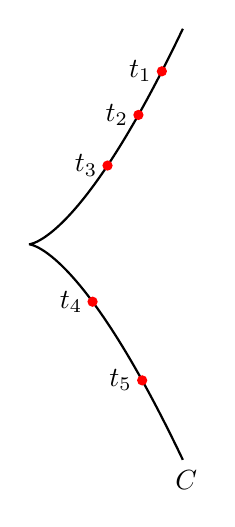
\begin{tikzpicture}[thick]
  \draw [domain=0:1.4, samples=100] 
  plot ({\x^2}, {\x^3} )
  plot ({\x^2}, {-\x^3} );
  \draw (2, -3) node {$C$};
  \draw[red, fill] (1.3^2, 1.3^3) circle (0.05) node [black, left] {$t_1$};
  \draw[red, fill] (1.18^2, 1.18^3) circle (0.05) node [black, left] {$t_2$};
  \draw[red, fill] (1.0^2, 1.0^3) circle (0.05) node [black, left] {$t_3$};
  \draw[red, fill] (1.2^2, -1.2^3) circle (0.05) node [black, left] {$t_5$};
  \draw[red, fill] (0.9^2, -0.9^3) circle (0.05) node [black, left] {$t_4$};
\end{tikzpicture}

%%% Local Variables:
%%% mode: latex
%%% TeX-master: "../main"
%%% End:
